% Options for packages loaded elsewhere
\PassOptionsToPackage{unicode}{hyperref}
\PassOptionsToPackage{hyphens}{url}
%
\documentclass[
]{book}
\usepackage{amsmath,amssymb}
\usepackage{iftex}
\ifPDFTeX
  \usepackage[T1]{fontenc}
  \usepackage[utf8]{inputenc}
  \usepackage{textcomp} % provide euro and other symbols
\else % if luatex or xetex
  \usepackage{unicode-math} % this also loads fontspec
  \defaultfontfeatures{Scale=MatchLowercase}
  \defaultfontfeatures[\rmfamily]{Ligatures=TeX,Scale=1}
\fi
\usepackage{lmodern}
\ifPDFTeX\else
  % xetex/luatex font selection
\fi
% Use upquote if available, for straight quotes in verbatim environments
\IfFileExists{upquote.sty}{\usepackage{upquote}}{}
\IfFileExists{microtype.sty}{% use microtype if available
  \usepackage[]{microtype}
  \UseMicrotypeSet[protrusion]{basicmath} % disable protrusion for tt fonts
}{}
\makeatletter
\@ifundefined{KOMAClassName}{% if non-KOMA class
  \IfFileExists{parskip.sty}{%
    \usepackage{parskip}
  }{% else
    \setlength{\parindent}{0pt}
    \setlength{\parskip}{6pt plus 2pt minus 1pt}}
}{% if KOMA class
  \KOMAoptions{parskip=half}}
\makeatother
\usepackage{xcolor}
\usepackage{color}
\usepackage{fancyvrb}
\newcommand{\VerbBar}{|}
\newcommand{\VERB}{\Verb[commandchars=\\\{\}]}
\DefineVerbatimEnvironment{Highlighting}{Verbatim}{commandchars=\\\{\}}
% Add ',fontsize=\small' for more characters per line
\usepackage{framed}
\definecolor{shadecolor}{RGB}{248,248,248}
\newenvironment{Shaded}{\begin{snugshade}}{\end{snugshade}}
\newcommand{\AlertTok}[1]{\textcolor[rgb]{0.94,0.16,0.16}{#1}}
\newcommand{\AnnotationTok}[1]{\textcolor[rgb]{0.56,0.35,0.01}{\textbf{\textit{#1}}}}
\newcommand{\AttributeTok}[1]{\textcolor[rgb]{0.13,0.29,0.53}{#1}}
\newcommand{\BaseNTok}[1]{\textcolor[rgb]{0.00,0.00,0.81}{#1}}
\newcommand{\BuiltInTok}[1]{#1}
\newcommand{\CharTok}[1]{\textcolor[rgb]{0.31,0.60,0.02}{#1}}
\newcommand{\CommentTok}[1]{\textcolor[rgb]{0.56,0.35,0.01}{\textit{#1}}}
\newcommand{\CommentVarTok}[1]{\textcolor[rgb]{0.56,0.35,0.01}{\textbf{\textit{#1}}}}
\newcommand{\ConstantTok}[1]{\textcolor[rgb]{0.56,0.35,0.01}{#1}}
\newcommand{\ControlFlowTok}[1]{\textcolor[rgb]{0.13,0.29,0.53}{\textbf{#1}}}
\newcommand{\DataTypeTok}[1]{\textcolor[rgb]{0.13,0.29,0.53}{#1}}
\newcommand{\DecValTok}[1]{\textcolor[rgb]{0.00,0.00,0.81}{#1}}
\newcommand{\DocumentationTok}[1]{\textcolor[rgb]{0.56,0.35,0.01}{\textbf{\textit{#1}}}}
\newcommand{\ErrorTok}[1]{\textcolor[rgb]{0.64,0.00,0.00}{\textbf{#1}}}
\newcommand{\ExtensionTok}[1]{#1}
\newcommand{\FloatTok}[1]{\textcolor[rgb]{0.00,0.00,0.81}{#1}}
\newcommand{\FunctionTok}[1]{\textcolor[rgb]{0.13,0.29,0.53}{\textbf{#1}}}
\newcommand{\ImportTok}[1]{#1}
\newcommand{\InformationTok}[1]{\textcolor[rgb]{0.56,0.35,0.01}{\textbf{\textit{#1}}}}
\newcommand{\KeywordTok}[1]{\textcolor[rgb]{0.13,0.29,0.53}{\textbf{#1}}}
\newcommand{\NormalTok}[1]{#1}
\newcommand{\OperatorTok}[1]{\textcolor[rgb]{0.81,0.36,0.00}{\textbf{#1}}}
\newcommand{\OtherTok}[1]{\textcolor[rgb]{0.56,0.35,0.01}{#1}}
\newcommand{\PreprocessorTok}[1]{\textcolor[rgb]{0.56,0.35,0.01}{\textit{#1}}}
\newcommand{\RegionMarkerTok}[1]{#1}
\newcommand{\SpecialCharTok}[1]{\textcolor[rgb]{0.81,0.36,0.00}{\textbf{#1}}}
\newcommand{\SpecialStringTok}[1]{\textcolor[rgb]{0.31,0.60,0.02}{#1}}
\newcommand{\StringTok}[1]{\textcolor[rgb]{0.31,0.60,0.02}{#1}}
\newcommand{\VariableTok}[1]{\textcolor[rgb]{0.00,0.00,0.00}{#1}}
\newcommand{\VerbatimStringTok}[1]{\textcolor[rgb]{0.31,0.60,0.02}{#1}}
\newcommand{\WarningTok}[1]{\textcolor[rgb]{0.56,0.35,0.01}{\textbf{\textit{#1}}}}
\usepackage{longtable,booktabs,array}
\usepackage{calc} % for calculating minipage widths
% Correct order of tables after \paragraph or \subparagraph
\usepackage{etoolbox}
\makeatletter
\patchcmd\longtable{\par}{\if@noskipsec\mbox{}\fi\par}{}{}
\makeatother
% Allow footnotes in longtable head/foot
\IfFileExists{footnotehyper.sty}{\usepackage{footnotehyper}}{\usepackage{footnote}}
\makesavenoteenv{longtable}
\usepackage{graphicx}
\makeatletter
\def\maxwidth{\ifdim\Gin@nat@width>\linewidth\linewidth\else\Gin@nat@width\fi}
\def\maxheight{\ifdim\Gin@nat@height>\textheight\textheight\else\Gin@nat@height\fi}
\makeatother
% Scale images if necessary, so that they will not overflow the page
% margins by default, and it is still possible to overwrite the defaults
% using explicit options in \includegraphics[width, height, ...]{}
\setkeys{Gin}{width=\maxwidth,height=\maxheight,keepaspectratio}
% Set default figure placement to htbp
\makeatletter
\def\fps@figure{htbp}
\makeatother
\setlength{\emergencystretch}{3em} % prevent overfull lines
\providecommand{\tightlist}{%
  \setlength{\itemsep}{0pt}\setlength{\parskip}{0pt}}
\setcounter{secnumdepth}{5}
\usepackage{booktabs}
\ifLuaTeX
  \usepackage{selnolig}  % disable illegal ligatures
\fi
\usepackage[]{natbib}
\bibliographystyle{plainnat}
\IfFileExists{bookmark.sty}{\usepackage{bookmark}}{\usepackage{hyperref}}
\IfFileExists{xurl.sty}{\usepackage{xurl}}{} % add URL line breaks if available
\urlstyle{same}
\hypersetup{
  pdftitle={Creating Migratory Networks in R: mignette},
  pdfauthor={Matt DeSaix},
  hidelinks,
  pdfcreator={LaTeX via pandoc}}

\title{Creating Migratory Networks in R: mignette}
\author{Matt DeSaix}
\date{2023-08-20}

\begin{document}
\maketitle

{
\setcounter{tocdepth}{1}
\tableofcontents
}
\hypertarget{introduction}{%
\chapter{Introduction}\label{introduction}}

This vignette outlines how to create migratory networks using the R package \texttt{mignette} (\textbf{mig}ratory \textbf{net}work \textbf{t}ools \textbf{e}nsemble). \texttt{mignette} was developed to facilitate conservation and management decision-making for migratory wildlife populations using migratory networks \citep{ruegg2020genoscape, taylor2010population}. The core function of \texttt{mignette} is to model the connectivity of populations across different stages of the annual cycle. To model these migratory networks in \texttt{mignette}, users need to provide:

\begin{enumerate}
\def\labelenumi{\arabic{enumi}.}
\tightlist
\item
  The number of individuals connecting migratory populations from two stages of the annual cycle
\item
  Relative abundance data for the populations
\end{enumerate}

We designed \texttt{mignette} specifically for use with population assignment data from genetic markers \citep{ruegg2014mapping, desaix2019population}, and we use genetic markers to delineate breeding populations (i.e., nodes in the migratory network model). We have since extended \texttt{mignette} to be able to model migratory networks that include geolocator data for assignment. While it is outside the scope of \texttt{mignette} for providing an exhaustive tool set of methods to delineate these nodes, given our focus on the use of genetic data, we provide examples and resources for users to delineate breeding populations from genetic data. For nonbreeding populations, we delineate these spatially by \emph{ecoregions} ADD LINK TO ECOREGION DATA SOURCE.

We anticipate users of \texttt{mignette} to be interested in modelling migratory networks for a wide-range of taxa, therefore users can provide relative abundance information from any data source. However, we also provide information on obtaining relative abundance for bird data from \href{https://ebird.org/science/status-and-trends}{eBird} and have developed tools in \texttt{mignette} to facilitate the calculation of relative abundance values.

For an introductory demonstration of creating a migratory network with \texttt{mignette}, see the \protect\hyperlink{quickstart}{quick start example}. Subsequent chapters of the vignette provide more detailed instructions and examples for delineating nodes (populations in the network model), calculating relative abundance for nodes, and running and visualizing the network model.

\hypertarget{installation}{%
\section{Installation}\label{installation}}

You can install the development version of \texttt{mignette} from GitHub with:

\begin{Shaded}
\begin{Highlighting}[]
\CommentTok{\# install.packages("remotes")}
\NormalTok{remotes}\SpecialCharTok{::}\FunctionTok{install\_github}\NormalTok{(}\StringTok{"mgdesaix/mignette"}\NormalTok{)}
\end{Highlighting}
\end{Shaded}

The migratory network model will be run using R packages that run JAGS (Just Another Gibbs Sampler). JAGS is a specific software for conducting analysis of Bayesian hierarchical models using Markov Chain Monte Carlo simulation. JAGS can be \href{https://mcmc-jags.sourceforge.io/}{downloaded here}

The primary packages for this vignette are:

\begin{Shaded}
\begin{Highlighting}[]
\FunctionTok{library}\NormalTok{(mignette)}
\FunctionTok{library}\NormalTok{(sf)}
\FunctionTok{library}\NormalTok{(terra)}
\FunctionTok{library}\NormalTok{(tidyverse)}
\FunctionTok{library}\NormalTok{(ebirdst) }\CommentTok{\# for avian abundance data from eBird Status and Trends}
\FunctionTok{library}\NormalTok{(rjags) }\CommentTok{\# for network model}
\FunctionTok{library}\NormalTok{(jagsUI) }\CommentTok{\# for network model}
\FunctionTok{library}\NormalTok{(ggnewscale) }\CommentTok{\# for network visualization}
\FunctionTok{library}\NormalTok{(tidyterra) }\CommentTok{\# for plotting terra objects with ggplot}
\end{Highlighting}
\end{Shaded}

As \texttt{mignette} makes use of the \texttt{terra} package, all raster and vector (e.g., polygons) are provided as \emph{SpatRaster} and \emph{SpatVector} objects. See the \texttt{terra} package for more details on these types of objects in R.

\hypertarget{quickstart}{%
\chapter{Quick start example}\label{quickstart}}

Here, we demonstrate a quick example of how to create a migratory network when the user has all of the data required. To run this tutorial, load the following packages:

\begin{Shaded}
\begin{Highlighting}[]
\FunctionTok{library}\NormalTok{(tidyverse)}
\FunctionTok{library}\NormalTok{(mignette)}
\FunctionTok{library}\NormalTok{(rjags)}
\FunctionTok{library}\NormalTok{(jagsUI)}
\FunctionTok{library}\NormalTok{(ggnewscale)}
\end{Highlighting}
\end{Shaded}

The data required are:

\begin{itemize}
\tightlist
\item
  Relative abundance matrix for each node
\item
  Assignment matrix of individuals among nodes
\end{itemize}

We provide an example of these data in \texttt{mignette}, with assignment data from 3 populations from the breeding range (WB = Western Boreal, NT = Northern Temperate, ST = Southern Temperate) and nonbreeding range (ALM = Atlantic Lowland Mexico, CAR = Caribbean, AONU = Amazon/Orinoco-Northern Uplands) of the American Redstart (\emph{Setophaga ruticilla}). The assignment matrix specifies the number of individuals that have been sampled or detected that migrate between different populations (i.e.~\emph{connect} the nodes).

\begin{Shaded}
\begin{Highlighting}[]
\NormalTok{mignette}\SpecialCharTok{::}\NormalTok{amre\_assign}
\end{Highlighting}
\end{Shaded}

\begin{tabular}{l|r|r|r|r|r}
\hline
Breeding & CAR & AONU & ALM & HCA & LCA\\
\hline
BR & 2 & 0 & 0 & 0 & 0\\
\hline
MP & 0 & 9 & 0 & 0 & 0\\
\hline
NT & 54 & 0 & 3 & 0 & 0\\
\hline
ST & 12 & 12 & 0 & 4 & 1\\
\hline
WB & 1 & 0 & 19 & 1 & 13\\
\hline
\end{tabular}

Assignment data input into \texttt{mignette} needs to follow the above format, where the first column specifies breeding population IDs while subsequent columns are the nonbreeding populations.

We also provide the relative abundance of these populations:

\begin{Shaded}
\begin{Highlighting}[]
\NormalTok{mignette}\SpecialCharTok{::}\NormalTok{amre\_abundance}
\end{Highlighting}
\end{Shaded}

\begin{tabular}{l|r}
\hline
Population & Relative\_abundance\\
\hline
BR & 2403\\
\hline
ST & 9419\\
\hline
MP & 19011\\
\hline
NT & 72147\\
\hline
WB & 26080\\
\hline
HCA & 326\\
\hline
AONU & 1139\\
\hline
LCA & 2802\\
\hline
ALM & 3169\\
\hline
CAR & 7987\\
\hline
\end{tabular}

The \emph{relative abundance} data needs to follow the above format for input into \texttt{mignette} functions with population IDs (same names as in the \emph{assignment} file) in the first column and relative abundance values in the second column. Column names can follow any naming convention when inputting these data into \texttt{mignette}.

For the following functions, we specify the order of the populations we are using for the model. Here, we are just ordering populations geographically by longitude to facilitate straightforward interpretation of the output.

\begin{Shaded}
\begin{Highlighting}[]
\NormalTok{bnode\_names }\OtherTok{\textless{}{-}} \FunctionTok{c}\NormalTok{(}\StringTok{"WB"}\NormalTok{, }\StringTok{"BR"}\NormalTok{, }\StringTok{"NT"}\NormalTok{, }\StringTok{"ST"}\NormalTok{, }\StringTok{"MP"}\NormalTok{)}
\NormalTok{wnode\_names }\OtherTok{\textless{}{-}} \FunctionTok{c}\NormalTok{(}\StringTok{"ALM"}\NormalTok{, }\StringTok{"LCA"}\NormalTok{, }\StringTok{"HCA"}\NormalTok{, }\StringTok{"CAR"}\NormalTok{, }\StringTok{"AONU"}\NormalTok{)}
\end{Highlighting}
\end{Shaded}

The following code provides the necessary data to run the JAGS model. To create the migratory network, the user first creates a text file specifying the JAGS model to be used, providing the name of the file to be saved (\texttt{base\_filename}) and the type of model type (\texttt{model\_type}). Currently \texttt{mignette} supports two model types based on the type of data used to determine assignment of individuals: \texttt{1} indicates that only genetic data were used for assignment, and \texttt{2} indicates that there's assignment data from both genetic and geolocator data. Here, the example only uses genetic data. \texttt{get\_jags\_model()} saves a \texttt{.txt} file with the \texttt{base\_filename} and stores that name as a variable for use in JAGS. We also specify the desired order of the breeding populations (\texttt{bnode\_names}) and the nonbreeding populations (\texttt{wnode\_names}). Finally, we use these as input into the function \texttt{get\_jags\_data()} to prepare the data appropriately for the model.

\begin{Shaded}
\begin{Highlighting}[]
\NormalTok{base\_filename }\OtherTok{\textless{}{-}}\NormalTok{ mignette}\SpecialCharTok{::}\FunctionTok{get\_jags\_model}\NormalTok{(}\AttributeTok{base\_filename =} \StringTok{"amre.genetic.model"}\NormalTok{, }\AttributeTok{model\_type =} \DecValTok{1}\NormalTok{)}
\NormalTok{jags\_data }\OtherTok{\textless{}{-}}\NormalTok{ mignette}\SpecialCharTok{::}\FunctionTok{get\_jags\_data}\NormalTok{(}\AttributeTok{abundance =}\NormalTok{ mignette}\SpecialCharTok{::}\NormalTok{amre\_abundance, }
                           \AttributeTok{assignment =}\NormalTok{ mignette}\SpecialCharTok{::}\NormalTok{amre\_assign,}
                           \AttributeTok{bnode\_names =}\NormalTok{ bnode\_names, }
                           \AttributeTok{wnode\_names =}\NormalTok{ wnode\_names)}
\end{Highlighting}
\end{Shaded}

Now the user can use the output of \texttt{jags\_data} into JAGS to run the actual model:

\begin{Shaded}
\begin{Highlighting}[]
\NormalTok{parameters }\OtherTok{\textless{}{-}} \FunctionTok{c}\NormalTok{(}\StringTok{"conn\_g"}\NormalTok{)}
\NormalTok{ni }\OtherTok{\textless{}{-}} \DecValTok{500000}
\NormalTok{nt }\OtherTok{\textless{}{-}} \DecValTok{4}
\NormalTok{nb }\OtherTok{\textless{}{-}} \DecValTok{100000}
\NormalTok{nc }\OtherTok{\textless{}{-}} \DecValTok{2}
\NormalTok{jags\_out }\OtherTok{\textless{}{-}} \FunctionTok{autojags}\NormalTok{(jags\_data, }\AttributeTok{inits=}\ConstantTok{NULL}\NormalTok{, parameters, }\FunctionTok{paste0}\NormalTok{(base\_filename,}\StringTok{".txt"}\NormalTok{),}
                      \AttributeTok{n.chains =}\NormalTok{ nc, }\AttributeTok{n.thin =}\NormalTok{nt, }\AttributeTok{iter.increment=}\NormalTok{ni,}
                      \AttributeTok{max.iter =}\NormalTok{ ni}\SpecialCharTok{*}\DecValTok{50}\SpecialCharTok{+}\NormalTok{nb, }\AttributeTok{n.burnin =}\NormalTok{ nb,}
                      \AttributeTok{n.adapt=} \ConstantTok{NULL}\NormalTok{, }\AttributeTok{parallel=}\ConstantTok{TRUE}\NormalTok{)}
\NormalTok{amre\_conn }\OtherTok{\textless{}{-}}\NormalTok{ jags\_out}\SpecialCharTok{$}\NormalTok{mean}\SpecialCharTok{$}\NormalTok{conn\_g}
\end{Highlighting}
\end{Shaded}

The connectivity between the nodes is provided by the \texttt{conn\_g} parameter of the model, which is accessed from the above code. We provide this output for the example as well with \texttt{mignette::amre\_conn}. We also provide functions for basic visualization of the network. A threshold (\texttt{connected\_tol}) can be set to remove very weak connectivity for better visualizing the network as shown below.

\begin{Shaded}
\begin{Highlighting}[]
\CommentTok{\# set threshold for not visualizing minimal connectivity}
\NormalTok{net }\OtherTok{\textless{}{-}}\NormalTok{ mignette}\SpecialCharTok{::}\FunctionTok{net\_create}\NormalTok{(mignette}\SpecialCharTok{::}\NormalTok{amre\_conn, }
                            \AttributeTok{node.names =} \FunctionTok{list}\NormalTok{(bnode\_names, wnode\_names),}
                            \AttributeTok{connected\_tol =} \FloatTok{0.02}\NormalTok{)}
\CommentTok{\#set the display size range for nodes (min and max), default 1{-}10}
\NormalTok{net}\SpecialCharTok{$}\NormalTok{display\_par}\SpecialCharTok{$}\NormalTok{node\_size\_scale}\OtherTok{\textless{}{-}}\FunctionTok{c}\NormalTok{(}\DecValTok{5}\NormalTok{,}\DecValTok{20}\NormalTok{)}
\CommentTok{\#set the display size range for edges (min and max), default 1{-}10}
\NormalTok{net}\SpecialCharTok{$}\NormalTok{display\_par}\SpecialCharTok{$}\NormalTok{edge\_size\_scale}\OtherTok{\textless{}{-}}\FunctionTok{c}\NormalTok{(}\DecValTok{1}\NormalTok{,}\DecValTok{5}\NormalTok{)}
\FunctionTok{plot}\NormalTok{(mignette}\SpecialCharTok{::}\FunctionTok{net\_draw}\NormalTok{(net))}
\end{Highlighting}
\end{Shaded}

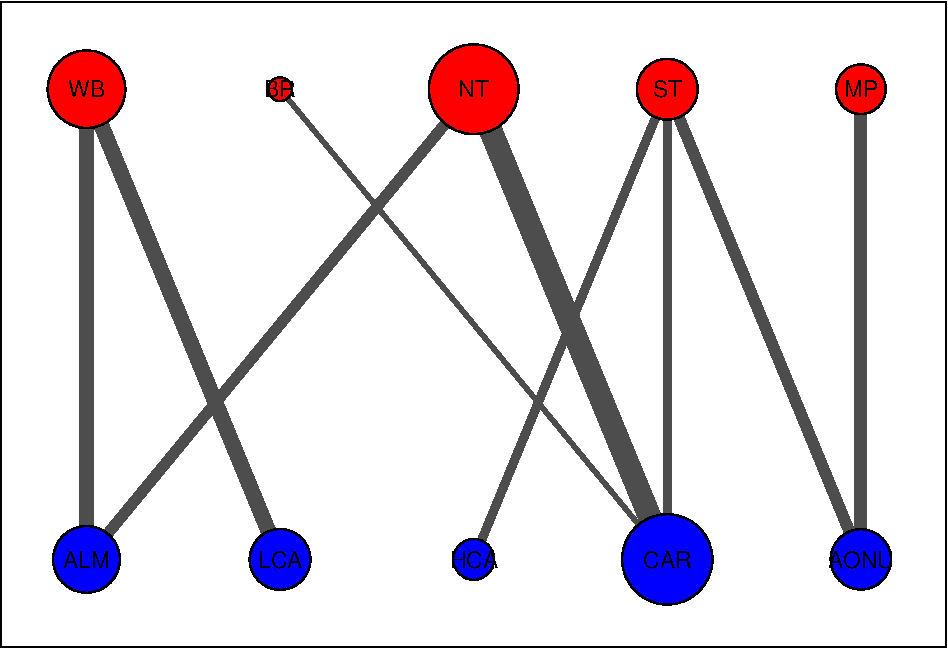
\includegraphics{Mignette_files/figure-latex/unnamed-chunk-5-1.pdf}

In this visualization, node size corresponds to the amount of connectivity with that population and edge size corresponds to the amount of connectivity between the populations. By default, breeding populations are in the top row (red) and nonbreeding/wintering populations are in the bottom row (blue).

This sums up the basics of creating and visualizing a migratory network. We encourage users to explore and build upon the visualization tools we provide (e.g.~overlay the migratory networks on geographic ranges) - the options are endless, enjoy!

\hypertarget{breeding}{%
\chapter{Breeding nodes}\label{breeding}}

Delineating breeding nodes is necessary for our migratory network model for both 1) assignment among populations, and 2) specifying a region for relative abundance. Here, we show how breeding nodes can be delineated by genetically distinct populations on the breeding grounds. In this example, we'll show how to use \href{https://ebird.org/science/status-and-trends}{eBird Status and Trends} data to specify the breeding range and then use genetic data from admixture analyses to specify the spatial extent of the breeding nodes.

\hypertarget{ebirdst}{%
\section{ebirdst}\label{ebirdst}}

In our migratory network analyses, the \href{https://science.ebird.org/en/status-and-trends}{eBird Status and Trends} data is used to delineate the different stages of the annual cycle. Prior to doing anything with eBird Status and Trends data, you will need to download the \texttt{ebirdst} package, and then get access to the data. \textbf{You will need to follow the most up-to-date instructions from the \texttt{ebirdst} developers for getting the abundance data. Currently, that information is here: \url{https://ebird.github.io/ebirdst/}}

To download the package:

\begin{Shaded}
\begin{Highlighting}[]
\CommentTok{\# install.packages("remotes")}
\NormalTok{remotes}\SpecialCharTok{::}\FunctionTok{install\_github}\NormalTok{(}\StringTok{"CornellLabofOrnithology/ebirdst"}\NormalTok{)}
\end{Highlighting}
\end{Shaded}

Then, get access to \texttt{ebirdst} data at \url{https://ebird.org/st/request}. You will receive a key to download \texttt{ebirdst} data and you can enter that key in R:

\begin{Shaded}
\begin{Highlighting}[]
\NormalTok{ebirdst}\SpecialCharTok{::}\FunctionTok{set\_ebirdst\_access\_key}\NormalTok{(}\StringTok{"XXXXX"}\NormalTok{)}
\end{Highlighting}
\end{Shaded}

where \texttt{"XXXXX"} is the key.

By following instructions from the \texttt{ebirdst} developers, you can obtain polygons of the breeding and nonbreeding ranges of avian species (see \url{https://ebird.github.io/ebirdst/} for details).

\hypertarget{creating-the-genoscape}{%
\section{Creating the genoscape}\label{creating-the-genoscape}}

A genoscape is the collection of genetically distinct populations that make up a species' range \citep{ruegg2021american}. Typically, for migratory species, the genoscape describes this population structure on the breeding range because the nonbreeding populations can can contain individuals from different breeding populations.

We will outline the main genoscape creation steps here, but full instructions on creating a genoscape map can be found in Eric Anderson's Github project \href{https://github.com/eriqande/make-a-BGP-map}{Make a Bird Genoscape Project map}. The input data needed for a genoscape are:

\begin{itemize}
\tightlist
\item
  Individual Q-value matrix
\item
  Lat/lon matrix of individuals
\item
  Breeding range polygon
\end{itemize}

The Q-value matrix is obtained from individual admixture analyses (e.g.~Structure, Admixture, \texttt{snmf} fuction from the LEA R-package). Latitude/longitude coordinates are for the individual samples used in the Q-value matrix. Breeding range polygons can be obtained from \texttt{ebirdst} (see previous section).

The \texttt{amre\_breeding\_data} data set provides admixture results (Q-values) for five genetic clusters for American Redstart (DeSaix et al.~2023) and metadata for the sampled individuals.

\begin{Shaded}
\begin{Highlighting}[]
\NormalTok{Q\_matrix }\OtherTok{\textless{}{-}}\NormalTok{ mignette}\SpecialCharTok{::}\NormalTok{amre\_breeding\_data }\SpecialCharTok{\%\textgreater{}\%}
\NormalTok{  dplyr}\SpecialCharTok{::}\FunctionTok{select}\NormalTok{(WB, BR, NT, ST, MP) }\SpecialCharTok{\%\textgreater{}\%}
  \FunctionTok{as.matrix}\NormalTok{()}

\NormalTok{coords }\OtherTok{\textless{}{-}}\NormalTok{ mignette}\SpecialCharTok{::}\NormalTok{amre\_breeding\_data }\SpecialCharTok{\%\textgreater{}\%}
\NormalTok{  dplyr}\SpecialCharTok{::}\FunctionTok{select}\NormalTok{(Lon, Lat) }\SpecialCharTok{\%\textgreater{}\%}
  \FunctionTok{as.matrix}\NormalTok{()}
\end{Highlighting}
\end{Shaded}

The larger data objects in \texttt{mignette} are stored in \texttt{extdata}:

\begin{Shaded}
\begin{Highlighting}[]
\NormalTok{breeding\_range }\OtherTok{\textless{}{-}} \FunctionTok{system.file}\NormalTok{(}\StringTok{"extdata"}\NormalTok{, }\StringTok{"amre\_breeding\_range.Rds"}\NormalTok{, }\AttributeTok{package =} \StringTok{"mignette"}\NormalTok{) }\SpecialCharTok{\%\textgreater{}\%}
\NormalTok{  terra}\SpecialCharTok{::}\FunctionTok{vect}\NormalTok{()}
  
\NormalTok{breeding\_range\_st }\OtherTok{\textless{}{-}}\NormalTok{ sf}\SpecialCharTok{::}\FunctionTok{st\_as\_sf}\NormalTok{(mignette}\SpecialCharTok{::}\NormalTok{amre\_breeding\_range) }\CommentTok{\# tess3Q\_map\_rasters function requires sf objects, not terra}
\end{Highlighting}
\end{Shaded}

We will also specify custom colors to correspond to the published genoscape.

\begin{Shaded}
\begin{Highlighting}[]
\NormalTok{cluster\_colors }\OtherTok{\textless{}{-}}  \FunctionTok{c}\NormalTok{(}
  \StringTok{\textasciigrave{}}\AttributeTok{ST}\StringTok{\textasciigrave{}} \OtherTok{=} \StringTok{"\#FF99FF"}\NormalTok{, }\CommentTok{\# pink/Southern Temperate}
  \StringTok{\textasciigrave{}}\AttributeTok{BR}\StringTok{\textasciigrave{}} \OtherTok{=} \StringTok{"\#3399FF"}\NormalTok{, }\CommentTok{\# blue/Basin Rockies}
  \StringTok{\textasciigrave{}}\AttributeTok{NT}\StringTok{\textasciigrave{}} \OtherTok{=} \StringTok{"\#FFFF33"}\NormalTok{, }\CommentTok{\# yellow/Northern Temperate}
  \StringTok{\textasciigrave{}}\AttributeTok{WB}\StringTok{\textasciigrave{}} \OtherTok{=} \StringTok{"\#339933"}\NormalTok{, }\CommentTok{\# green/Western Boreal}
  \StringTok{\textasciigrave{}}\AttributeTok{MP}\StringTok{\textasciigrave{}} \OtherTok{=} \StringTok{"\#CC0033"} \CommentTok{\# red/Maritime Provinces}
\NormalTok{) }
\end{Highlighting}
\end{Shaded}

We will use a \href{https://github.com/eriqande/TESS3_encho_sen}{modified version} of the \texttt{tess3r} package to create the genoscape rasters.

\begin{Shaded}
\begin{Highlighting}[]
\CommentTok{\# remotes::install\_github("eriqande/TESS3\_encho\_sen")}
\NormalTok{amre\_genoscape }\OtherTok{\textless{}{-}}\NormalTok{ tess3r}\SpecialCharTok{::}\FunctionTok{tess3Q\_map\_rasters}\NormalTok{(}
  \AttributeTok{x =}\NormalTok{ Q\_matrix,}
  \AttributeTok{coord =}\NormalTok{ coords,}
  \AttributeTok{map.polygon =}\NormalTok{ breeding\_range\_st,}
  \AttributeTok{window =}\NormalTok{ sf}\SpecialCharTok{::}\FunctionTok{st\_bbox}\NormalTok{(breeding\_range\_st),}
  \AttributeTok{resolution =} \FunctionTok{c}\NormalTok{(}\DecValTok{300}\NormalTok{,}\DecValTok{300}\NormalTok{), }\CommentTok{\# if you want more cells in your raster, set higher}
  \AttributeTok{col.palette =}\NormalTok{ tess3r}\SpecialCharTok{::}\FunctionTok{CreatePalette}\NormalTok{(cluster\_colors, }\FunctionTok{length}\NormalTok{(cluster\_colors)), }
  \AttributeTok{method =} \StringTok{"map.max"}\NormalTok{, }
  \AttributeTok{interpol =}\NormalTok{ tess3r}\SpecialCharTok{::}\FunctionTok{FieldsKrigModel}\NormalTok{(}\DecValTok{10}\NormalTok{),  }
  \AttributeTok{main =} \StringTok{"Ancestry coefficients"}\NormalTok{,}
  \AttributeTok{xlab =} \StringTok{"Longitude"}\NormalTok{, }
  \AttributeTok{ylab =} \StringTok{"Latitude"}\NormalTok{, }
  \AttributeTok{cex =}\NormalTok{ .}\DecValTok{4}
\NormalTok{)}
\FunctionTok{names}\NormalTok{(amre\_genoscape) }\OtherTok{\textless{}{-}} \FunctionTok{colnames}\NormalTok{(Q\_matrix)}
\NormalTok{amre\_genoscape }\OtherTok{\textless{}{-}}\NormalTok{ terra}\SpecialCharTok{::}\FunctionTok{rast}\NormalTok{(amre\_genoscape) }\CommentTok{\# convert from rasterbrick to spatRaster}
\FunctionTok{crs}\NormalTok{(amre\_genoscape) }\OtherTok{\textless{}{-}} \StringTok{"EPSG:4326"} \CommentTok{\# Set CRS projection}
\end{Highlighting}
\end{Shaded}

Check out the resulting genoscape:

\begin{Shaded}
\begin{Highlighting}[]
\FunctionTok{plot}\NormalTok{(amre\_genoscape)}
\end{Highlighting}
\end{Shaded}

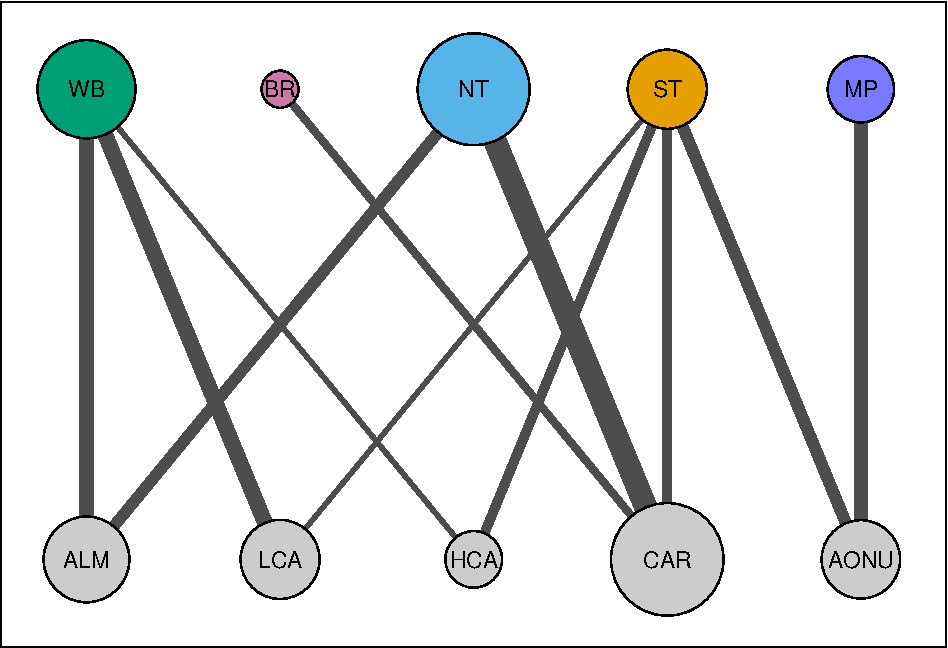
\includegraphics{Mignette_files/figure-latex/unnamed-chunk-7-1.pdf}

\textbf{STOP}

The rasters for the genoscape are all that are needed for obtaining information on relative abundance for the different populations. You can continue on to the \protect\hyperlink{abundance}{relative abundance chapter} if you are ready to do that with the genoscape. Or if you still need to create the wintering nodes, check out the next chapter on \protect\hyperlink{wintering}{wintering nodes}. The following section is not necessary for the migratory network but details how to covert genoscape rasters to polygons if the \texttt{mignette} user is interested in doing so.

\hypertarget{genoscape-polygons}{%
\subsection{Genoscape polygons}\label{genoscape-polygons}}

Using the genoscape rasters we will convert them to polygons, using the handy \texttt{scape\_to\_shape()} function. The \texttt{prob\_threshold} parameter specifies the value to determine if a raster cell is included in the polygon for that genoscape. This value should be customized for different species to check for overlap of genoscape polygons, which is not desirable. Setting too high of a threshold will create very small breeding nodes, while too low of a threshold will result in large, overlapping breeding nodes.

Check out the polygons

\begin{Shaded}
\begin{Highlighting}[]
\NormalTok{genoscape\_polygons }\OtherTok{\textless{}{-}}\NormalTok{ mignette}\SpecialCharTok{::}\FunctionTok{scape\_to\_shape}\NormalTok{(}\AttributeTok{x =}\NormalTok{ amre\_genoscape, }
                                               \AttributeTok{prob\_threshold =} \FloatTok{0.5}\NormalTok{)}
\end{Highlighting}
\end{Shaded}

\begin{verbatim}
## Spherical geometry (s2) switched off
\end{verbatim}

\begin{Shaded}
\begin{Highlighting}[]
\FunctionTok{ggplot}\NormalTok{() }\SpecialCharTok{+}
  \FunctionTok{geom\_sf}\NormalTok{(}\AttributeTok{data =}\NormalTok{ genoscape\_polygons,}\AttributeTok{alpha =} \FloatTok{0.75}\NormalTok{, }\FunctionTok{aes}\NormalTok{(}\AttributeTok{fill =}\NormalTok{ Cluster)) }\SpecialCharTok{+}
  \FunctionTok{scale\_fill\_manual}\NormalTok{(}\AttributeTok{values =}\NormalTok{ cluster\_colors) }\SpecialCharTok{+}
  \FunctionTok{theme\_bw}\NormalTok{()}
\end{Highlighting}
\end{Shaded}

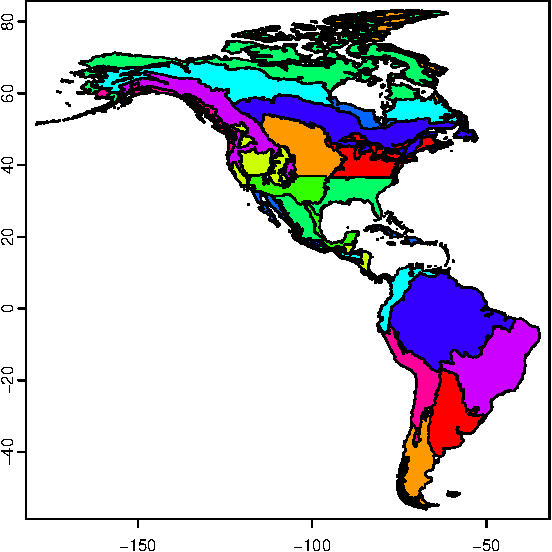
\includegraphics[width=0.7\linewidth]{Mignette_files/figure-latex/unnamed-chunk-9-1}

Note that the lower population membership probabilities occur at the boundaries of different populations, thereby making the polygons discontinuous compared to the entire range

Now on to creating the \protect\hyperlink{wintering}{wintering nodes}

\hypertarget{wintering}{%
\chapter{Nonbreeding nodes}\label{wintering}}

For the migratory networks, we will use ecoregions to define the nonbreeding nodes. However, other nonbreeding nodes could be defined by the user instead. If you already have polygons defining your nodes interest, then continue to the \protect\hyperlink{abundance}{relative abundance section}.

\hypertarget{subsetting-ecoregions}{%
\section{Subsetting ecoregions}\label{subsetting-ecoregions}}

The ecoregion data is derived from {[}provide link{]} and defines biogeographic regions in the Western Hemisphere. We provide these as external data stored as a SpatVector. We will intersect the ecoregions with the nonbreeding range of the American Redstart to identify all the ecoregions for this region.

\begin{Shaded}
\begin{Highlighting}[]
\FunctionTok{library}\NormalTok{(mignette)}
\FunctionTok{library}\NormalTok{(terra)}
\FunctionTok{library}\NormalTok{(tidyterra)}
\FunctionTok{library}\NormalTok{(tidyverse)}
\end{Highlighting}
\end{Shaded}

\begin{Shaded}
\begin{Highlighting}[]
\NormalTok{ecoregions }\OtherTok{\textless{}{-}} \FunctionTok{system.file}\NormalTok{(}\StringTok{"extdata"}\NormalTok{, }\StringTok{"ecoregions.Rds"}\NormalTok{,}
                          \AttributeTok{package =} \StringTok{"mignette"}\NormalTok{) }\SpecialCharTok{\%\textgreater{}\%}
\NormalTok{  terra}\SpecialCharTok{::}\FunctionTok{vect}\NormalTok{()}
\NormalTok{amre\_nonbreeding\_range }\OtherTok{\textless{}{-}} \FunctionTok{system.file}\NormalTok{(}\StringTok{"extdata"}\NormalTok{, }\StringTok{"amre\_nonbreeding\_range.Rds"}\NormalTok{,}
                                      \AttributeTok{package =} \StringTok{"mignette"}\NormalTok{) }\SpecialCharTok{\%\textgreater{}\%}
\NormalTok{  terra}\SpecialCharTok{::}\FunctionTok{vect}\NormalTok{()}

\NormalTok{amre\_nonbreeding\_ecoregions }\OtherTok{\textless{}{-}}\NormalTok{ terra}\SpecialCharTok{::}\FunctionTok{intersect}\NormalTok{(amre\_nonbreeding\_range, ecoregions)}

\FunctionTok{ggplot}\NormalTok{() }\SpecialCharTok{+}
\NormalTok{  tidyterra}\SpecialCharTok{::}\FunctionTok{geom\_spatvector}\NormalTok{(}\AttributeTok{data =}\NormalTok{ amre\_nonbreeding\_ecoregions, }
                  \FunctionTok{aes}\NormalTok{(}\AttributeTok{fill =}\NormalTok{ Region)) }\SpecialCharTok{+}
  \FunctionTok{theme\_bw}\NormalTok{()}
\end{Highlighting}
\end{Shaded}

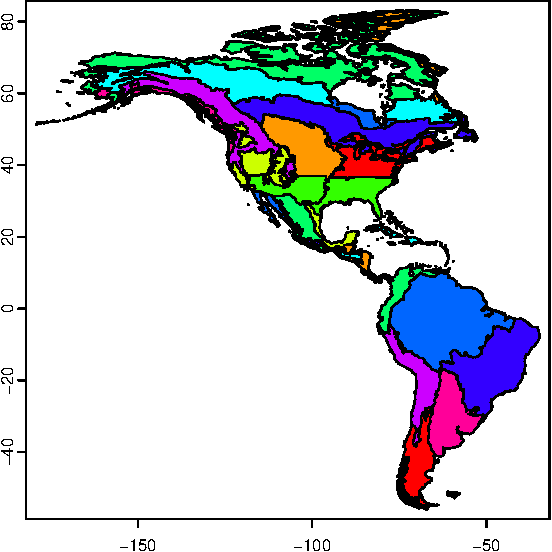
\includegraphics{Mignette_files/figure-latex/unnamed-chunk-11-1.pdf}

\hypertarget{select-sampled-regions}{%
\section{Select sampled regions}\label{select-sampled-regions}}

For the purpose of the migratory network, we are only interested in nonbreeding nodes for which we have sampled data. To identify these nodes, we will intersect our sampled nonbreeding individuals locations with the ecoregion data. Additionally, since sampling locations may fall just outside an ecoregion boundary (for example, imprecise coordinates along a coast) we will identify the ecoregions by selecting the \emph{nearest} ecoregion to a point.

\begin{Shaded}
\begin{Highlighting}[]
\NormalTok{nonbreeding\_coords }\OtherTok{\textless{}{-}}\NormalTok{ terra}\SpecialCharTok{::}\FunctionTok{vect}\NormalTok{(mignette}\SpecialCharTok{::}\NormalTok{amre\_nonbreeding\_data, }
                             \AttributeTok{geom=}\FunctionTok{c}\NormalTok{(}\StringTok{"Lon"}\NormalTok{, }\StringTok{"Lat"}\NormalTok{),}
                             \AttributeTok{crs =} \StringTok{"EPSG:4326"}\NormalTok{)}
\NormalTok{nonbreeding\_coords\_nearest }\OtherTok{\textless{}{-}}\NormalTok{ terra}\SpecialCharTok{::}\FunctionTok{nearest}\NormalTok{(nonbreeding\_coords,}
\NormalTok{                                        ecoregions,}
                                        \AttributeTok{centroids =} \ConstantTok{FALSE}\NormalTok{)}
\CommentTok{\# Add Region ID from original file for easier interpretation}
\NormalTok{nonbreeding\_coords\_nearest}\SpecialCharTok{$}\NormalTok{Region }\OtherTok{\textless{}{-}}\NormalTok{ ecoregions}\SpecialCharTok{$}\NormalTok{Region[nonbreeding\_coords\_nearest}\SpecialCharTok{$}\NormalTok{to\_id]}
\end{Highlighting}
\end{Shaded}

\begin{Shaded}
\begin{Highlighting}[]
\FunctionTok{table}\NormalTok{(nonbreeding\_coords\_nearest}\SpecialCharTok{$}\NormalTok{Region)}
\end{Highlighting}
\end{Shaded}

\begin{tabular}{l|r}
\hline
Var1 & Freq\\
\hline
Amazon/Orinoco-Northern Uplands & 21\\
\hline
Atlantic Lowland Mexico & 22\\
\hline
Caribbean & 69\\
\hline
Highland Central America & 5\\
\hline
Highland/Interior Mexico & 1\\
\hline
Lowland Central America & 14\\
\hline
Northern Andes & 3\\
\hline
\end{tabular}

For the migratory network, we also want sufficient sampling of a node for the model to be able to reach convergence. In the example above, we see ``Highland/Interior Mexico'' only has 1 sample and the ``Northern Andes'' only have 3 samples. Below, we use a cut off of a minimum of 4 samples to remove those ecoregions

\begin{Shaded}
\begin{Highlighting}[]
\NormalTok{cutoff }\OtherTok{\textless{}{-}} \DecValTok{4}

\NormalTok{ecoregions\_keep }\OtherTok{\textless{}{-}} \FunctionTok{data.frame}\NormalTok{(}\FunctionTok{table}\NormalTok{(nonbreeding\_coords\_nearest}\SpecialCharTok{$}\NormalTok{Region)) }\SpecialCharTok{\%\textgreater{}\%}
  \FunctionTok{filter}\NormalTok{(}\SpecialCharTok{!}\NormalTok{.[}\DecValTok{2}\NormalTok{] }\SpecialCharTok{\textless{}}\NormalTok{ cutoff) }\SpecialCharTok{\%\textgreater{}\%}
  \FunctionTok{pull}\NormalTok{(}\DecValTok{1}\NormalTok{) }\SpecialCharTok{\%\textgreater{}\%}
  \FunctionTok{as.character}\NormalTok{()}

\NormalTok{nonbreeding\_coords\_nearest\_subset }\OtherTok{\textless{}{-}}\NormalTok{ nonbreeding\_coords\_nearest[nonbreeding\_coords\_nearest}\SpecialCharTok{$}\NormalTok{Region }\SpecialCharTok{\%in\%}\NormalTok{ ecoregions\_keep]}
\NormalTok{nonbreeding\_regions\_subset }\OtherTok{\textless{}{-}}\NormalTok{ ecoregions[nonbreeding\_coords\_nearest\_subset]}
\end{Highlighting}
\end{Shaded}

This leaves us with a final set of our nonbreeding nodes and the samples associated with them:

\begin{Shaded}
\begin{Highlighting}[]
\FunctionTok{ggplot}\NormalTok{() }\SpecialCharTok{+}
  \FunctionTok{geom\_spatvector}\NormalTok{(}\AttributeTok{data =}\NormalTok{ nonbreeding\_regions\_subset, }\FunctionTok{aes}\NormalTok{(}\AttributeTok{fill =}\NormalTok{ Region)) }\SpecialCharTok{+}
  \FunctionTok{geom\_spatvector}\NormalTok{(}\AttributeTok{data =}\NormalTok{ nonbreeding\_coords\_nearest\_subset) }\SpecialCharTok{+}
  \FunctionTok{theme\_bw}\NormalTok{()}
\end{Highlighting}
\end{Shaded}

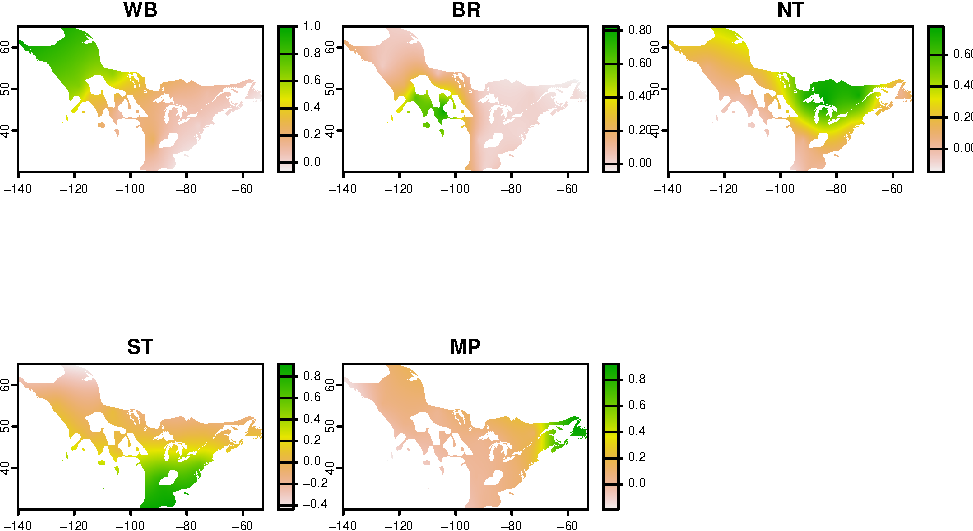
\includegraphics{Mignette_files/figure-latex/unnamed-chunk-15-1.pdf}

Now on to getting the \protect\hyperlink{assignment}{node assignment matrix}.

\hypertarget{assignment}{%
\chapter{Node assignment}\label{assignment}}

In \texttt{mignette}, node assignment data is one of the two main inputs into the migratory network model. Regardless of the methods used to collect these data, as input into the \texttt{mignette} migratory network model it needs to be in a specific format:

\begin{tabular}{l|r|r|r|r|r}
\hline
Breeding & CAR & AONU & ALM & HCA & LCA\\
\hline
BR & 2 & 0 & 0 & 0 & 0\\
\hline
MP & 0 & 9 & 0 & 0 & 0\\
\hline
NT & 54 & 0 & 3 & 0 & 0\\
\hline
ST & 12 & 12 & 0 & 4 & 1\\
\hline
WB & 1 & 0 & 19 & 1 & 13\\
\hline
\end{tabular}

The first column specifies the \emph{inferred} nodes in assignment. In the case of the genetic assignment data shown above, the breeding nodes are inferred from population assignment methods with individuals sampled from the nonbreeding range. The other column names refer to the nonbreeding node names, and the values are the number of individuals from a given nonbreeding node assigned to the respective breeding node specified by the row.

For the American Redstart example, we can get the assignment data in the format shown above based on population assignment data provided in \texttt{mignette} as well as the ecoregion information from the previous section.

The \texttt{amre\_nonbreeding\_range} data, from which we extracted the latitude and longitude coordinates of sampling locations to identify ecoregions in the previous section, also provides the breeding node assignment data from DeSaix et al.~(2023). Creating the \texttt{nonbreeding\_coords\_nearest} object retained the same row order of data as in the original \texttt{amre\_nonbreeding\_range}, thus we can combine these data in the following way. \textbf{Note:} We are manually combining these data without a \emph{join} by sample name or another identifier so it is always good to triple check that indeed the data are in the correct order when not using a join.

\begin{Shaded}
\begin{Highlighting}[]
\NormalTok{amre\_assign\_manual }\OtherTok{\textless{}{-}} \FunctionTok{tibble}\NormalTok{(}\StringTok{"Breeding"} \OtherTok{=}\NormalTok{ amre\_nonbreeding\_data}\SpecialCharTok{$}\NormalTok{Breeding\_assignment,}
                             \StringTok{"Nonbreeding"} \OtherTok{=}\NormalTok{ nonbreeding\_coords\_nearest}\SpecialCharTok{$}\NormalTok{Region) }\SpecialCharTok{\%\textgreater{}\%}
  \FunctionTok{filter}\NormalTok{(Nonbreeding }\SpecialCharTok{\%in\%}\NormalTok{ ecoregions\_keep) }\SpecialCharTok{\%\textgreater{}\%} \CommentTok{\# remove those nonbreeding nodes with \textless{}4 samples}
  \FunctionTok{group\_by}\NormalTok{(Breeding, Nonbreeding) }\SpecialCharTok{\%\textgreater{}\%}
  \FunctionTok{summarize}\NormalTok{(}\AttributeTok{N =} \FunctionTok{n}\NormalTok{(),}
            \AttributeTok{.groups =} \StringTok{"drop"}\NormalTok{) }\SpecialCharTok{\%\textgreater{}\%}
  \FunctionTok{pivot\_wider}\NormalTok{(}\AttributeTok{names\_from =}\NormalTok{ Nonbreeding, }\AttributeTok{values\_from =}\NormalTok{ N) }\SpecialCharTok{\%\textgreater{}\%}
  \FunctionTok{rename}\NormalTok{(}\StringTok{"AONU"} \OtherTok{=} \StringTok{"Amazon/Orinoco{-}Northern Uplands"}\NormalTok{,}
         \StringTok{"ALM"} \OtherTok{=} \StringTok{"Atlantic Lowland Mexico"}\NormalTok{,}
         \StringTok{"CAR"} \OtherTok{=} \StringTok{"Caribbean"}\NormalTok{,}
         \StringTok{"HCA"} \OtherTok{=} \StringTok{"Highland Central America"}\NormalTok{,}
         \StringTok{"LCA"} \OtherTok{=} \StringTok{"Lowland Central America"}\NormalTok{) }\SpecialCharTok{\%\textgreater{}\%}
  \FunctionTok{mutate}\NormalTok{(}\FunctionTok{across}\NormalTok{(}\FunctionTok{where}\NormalTok{(is.numeric), }\SpecialCharTok{\textasciitilde{}}\FunctionTok{ifelse}\NormalTok{(}\FunctionTok{is.na}\NormalTok{(.), }\DecValTok{0}\NormalTok{, .))) }\CommentTok{\# replace NAs with 0s}
\end{Highlighting}
\end{Shaded}

\begin{Shaded}
\begin{Highlighting}[]
\NormalTok{amre\_assign\_manual}
\end{Highlighting}
\end{Shaded}

\begin{tabular}{l|r|r|r|r|r}
\hline
Breeding & CAR & AONU & ALM & HCA & LCA\\
\hline
BR & 2 & 0 & 0 & 0 & 0\\
\hline
MP & 0 & 9 & 0 & 0 & 0\\
\hline
NT & 54 & 0 & 3 & 0 & 0\\
\hline
ST & 12 & 12 & 0 & 4 & 1\\
\hline
WB & 1 & 0 & 19 & 1 & 13\\
\hline
\end{tabular}

We can see that we have effectively mapped the breeding population assignment meta data to the correct ecoregion based on our individual's sampling location. Great!

Now on to getting the \protect\hyperlink{abundance}{relative abundance}.

\hypertarget{abundance}{%
\chapter{Relative Abundance}\label{abundance}}

Here, we calculate the relative abundance for the different nodes of the migratory network. The input data for this step are:

\begin{itemize}
\tightlist
\item
  Abundance data (Raster)
\item
  Population ranges (Raster or Vector)
\end{itemize}

Typically, the geographic range of a population will be stored as a vector (e.g., polygon), but in the case of a genoscape, the population ranges can be specified by a raster with q-values. For abundance data, we will use the \href{https://science.ebird.org/en/status-and-trends}{eBird Status and Trends} data which are obtained with the \href{https://cornelllabofornithology.github.io/ebirdst/}{ebirdst R package}, but any abundance data in a raster object can be used. \textbf{Note:} We do not provide the \texttt{ebirdst} data within \texttt{mignette} - these data are publicly available and licensed by the Cornell Lab of Ornithology and can be obtained by following the appropriate directions in the above links.

\hypertarget{get-relative-abundance-for-a-genoscape-raster}{%
\section{Get relative abundance for a genoscape (raster)}\label{get-relative-abundance-for-a-genoscape-raster}}

In the case of a \emph{genoscape} raster with q-values, we will convert the q-values to probabilities of a pixel belonging to that population which is used to weight the abundance values. This is done with a single function \texttt{get\_genoscape\_abunds()}, and outputs a two-column matrix with the population names and the relative abundance of each population. Below, we provide an example with the genoscape as a SpatRaster (\texttt{genoscape}) and the ebirdst abundance data as a SpatRaster (\texttt{abunds}; obtained from the links above).

\begin{Shaded}
\begin{Highlighting}[]
\NormalTok{genoscape\_abunds }\OtherTok{\textless{}{-}} \FunctionTok{get\_genoscape\_abunds}\NormalTok{(}\AttributeTok{genoscape =}\NormalTok{ amre\_genoscape, }\AttributeTok{abunds =}\NormalTok{ abunds)}
\end{Highlighting}
\end{Shaded}

\hypertarget{get-relative-abundance-for-a-vector}{%
\section{Get relative abundance for a vector}\label{get-relative-abundance-for-a-vector}}

In the case of vector file delineating populations, we sum abundance across the range of each population. This is done with a single function \texttt{get\_vector\_abunds()}, and outputs a two-column matrix with the population names and the relative abundance of each population. The example below provides the nonbreeding ecoregions file as a SpatVector (\texttt{winter\_regions}) and the ebirdst abundance data as a SpatRaster (\texttt{abunds})

\begin{Shaded}
\begin{Highlighting}[]
\NormalTok{winter\_abunds }\OtherTok{\textless{}{-}} \FunctionTok{get\_vector\_abunds}\NormalTok{(}\AttributeTok{populations =}\NormalTok{ nonbreeding\_regions\_subset, }\AttributeTok{abunds =}\NormalTok{ abunds)}
\end{Highlighting}
\end{Shaded}

\hypertarget{combine-the-abundance-data}{%
\section{Combine the abundance data}\label{combine-the-abundance-data}}

As you'll see in the next section, these data are one of the primary inputs into the migratory network model and we combine the relative abundance data sets across the breeding and nonbreeding nodes with the following code. The final product is what we provide in this package

\begin{Shaded}
\begin{Highlighting}[]
\NormalTok{amre\_abundance }\OtherTok{\textless{}{-}} \FunctionTok{rbind}\NormalTok{(genoscape\_abunds, winter\_abunds) }\SpecialCharTok{\%\textgreater{}\%}
  \FunctionTok{as\_tibble}\NormalTok{() }\SpecialCharTok{\%\textgreater{}\%}
  \FunctionTok{mutate}\NormalTok{(}\AttributeTok{Relative\_abundance =} \FunctionTok{round}\NormalTok{(}\FunctionTok{as.numeric}\NormalTok{(Relative\_abundance)))}
\NormalTok{amre\_abundance}
\end{Highlighting}
\end{Shaded}

\begin{tabular}{l|r}
\hline
Population & Relative\_abundance\\
\hline
BR & 2403\\
\hline
ST & 9419\\
\hline
MP & 19011\\
\hline
NT & 72147\\
\hline
WB & 26080\\
\hline
HCA & 326\\
\hline
AONU & 1139\\
\hline
LCA & 2802\\
\hline
ALM & 3169\\
\hline
CAR & 7987\\
\hline
\end{tabular}

Now on to creating the \protect\hyperlink{connectivity}{migratory network model}.

\hypertarget{connectivity}{%
\chapter{Migratory Network Model}\label{connectivity}}

\hypertarget{input-data}{%
\section{Input data}\label{input-data}}

The input data we need for the migratory network model are:

\begin{itemize}
\tightlist
\item
  Relative abundance matrix for each node
\item
  Assignment matrix of individuals among nodes
\end{itemize}

We demonstrate in the previous \protect\hyperlink{abundance}{relative abundance section} how to obtain the relative abundance data needed for the model. The relative abundance data need to be in the following format, with population IDs (same names as in the \emph{assignment} file) in the first column and relative abundance values in the second column. Column names can follow any naming convention when inputting these data into \texttt{mignette}.

\begin{tabular}{l|r}
\hline
Population & Relative\_abundance\\
\hline
BR & 2403\\
\hline
ST & 9419\\
\hline
MP & 19011\\
\hline
NT & 72147\\
\hline
WB & 26080\\
\hline
HCA & 326\\
\hline
AONU & 1139\\
\hline
LCA & 2802\\
\hline
ALM & 3169\\
\hline
CAR & 7987\\
\hline
\end{tabular}

For the assignment matrix, the input data needs to correspond to the following format:

\begin{tabular}{l|r|r|r|r|r}
\hline
Breeding & CAR & AONU & ALM & HCA & LCA\\
\hline
BR & 2 & 0 & 0 & 0 & 0\\
\hline
MP & 0 & 9 & 0 & 0 & 0\\
\hline
NT & 54 & 0 & 3 & 0 & 0\\
\hline
ST & 12 & 12 & 0 & 4 & 1\\
\hline
WB & 1 & 0 & 19 & 1 & 13\\
\hline
\end{tabular}

where the first column specifies breeding population IDs while subsequent columns are the nonbreeding populations. The values are the number of individuals that connect each node. Depending on the type of assignment data the \texttt{mignette} user has, individual data points may need to be associated with a specific population. For these types of basic spatial analyses, \texttt{mignette} users can check out the \texttt{sf} package, specifically the \texttt{st\_intersection()} function, or whatever geospatial tools they prefer to create these data. Once you have connectivity data in the above format, you can continue with the following sections.

For the following functions, we specify the order of the populations we are using for the model. Here, we are just ordering populations geographically by longitude to facilitate straightforward interpretation of the output.

\begin{Shaded}
\begin{Highlighting}[]
\NormalTok{bnode\_names }\OtherTok{\textless{}{-}} \FunctionTok{c}\NormalTok{(}\StringTok{"WB"}\NormalTok{, }\StringTok{"BR"}\NormalTok{, }\StringTok{"NT"}\NormalTok{, }\StringTok{"ST"}\NormalTok{, }\StringTok{"MP"}\NormalTok{)}
\NormalTok{wnode\_names }\OtherTok{\textless{}{-}} \FunctionTok{c}\NormalTok{(}\StringTok{"ALM"}\NormalTok{, }\StringTok{"LCA"}\NormalTok{, }\StringTok{"HCA"}\NormalTok{, }\StringTok{"CAR"}\NormalTok{, }\StringTok{"AONU"}\NormalTok{)}
\end{Highlighting}
\end{Shaded}

\hypertarget{migratory-network-model-jags}{%
\section{Migratory network model (JAGS)}\label{migratory-network-model-jags}}

\hypertarget{preparing-input-data}{%
\subsection{Preparing input data}\label{preparing-input-data}}

The following code provides the necessary data to run the JAGS model. To create the migratory network, the user first creates a text file specifying the JAGS model to be used, providing the name of the file to be saved (\texttt{base\_filename}) and the type of model type (\texttt{model\_type}). Currently \texttt{mignette} supports two model types based on the type of data used to determine assignment of individuals: \texttt{1} indicates that only genetic data were used for assignment, and \texttt{2} indicates that there's assignment data from both genetic and geolocator data. Here, the example only uses genetic data. \texttt{get\_jags\_model()} saves a \texttt{.txt} file with the \texttt{base\_filename} and stores that name as a variable for use in JAGS. We also specify the desired order of the breeding populations (\texttt{bnode\_names}) and the nonbreeding populations (\texttt{wnode\_names}). Finally, we use these as input into the function \texttt{get\_jags\_data()} to prepare the data appropriately for the model.

\begin{Shaded}
\begin{Highlighting}[]
\NormalTok{base\_filename }\OtherTok{\textless{}{-}}\NormalTok{ mignette}\SpecialCharTok{::}\FunctionTok{get\_jags\_model}\NormalTok{(}\AttributeTok{base\_filename =} \StringTok{"amre.genetic.model"}\NormalTok{, }\AttributeTok{model\_type =} \DecValTok{1}\NormalTok{)}
\NormalTok{jags\_data }\OtherTok{\textless{}{-}}\NormalTok{ mignette}\SpecialCharTok{::}\FunctionTok{get\_jags\_data}\NormalTok{(}\AttributeTok{abundance =}\NormalTok{ mignette}\SpecialCharTok{::}\NormalTok{amre\_abundance, }
                           \AttributeTok{assignment =}\NormalTok{ mignette}\SpecialCharTok{::}\NormalTok{amre\_assign,}
                           \AttributeTok{bnode\_names =}\NormalTok{ bnode\_names, }
                           \AttributeTok{wnode\_names =}\NormalTok{ wnode\_names)}
\end{Highlighting}
\end{Shaded}

\hypertarget{running-the-model}{%
\subsection{Running the model}\label{running-the-model}}

Now the user can use the output of \texttt{jags\_data} into JAGS to run the actual model:

\begin{Shaded}
\begin{Highlighting}[]
\NormalTok{parameters }\OtherTok{\textless{}{-}} \FunctionTok{c}\NormalTok{(}\StringTok{"conn\_g"}\NormalTok{)}
\NormalTok{ni }\OtherTok{\textless{}{-}} \DecValTok{500000}
\NormalTok{nt }\OtherTok{\textless{}{-}} \DecValTok{4}
\NormalTok{nb }\OtherTok{\textless{}{-}} \DecValTok{100000}
\NormalTok{nc }\OtherTok{\textless{}{-}} \DecValTok{2}
\NormalTok{jags\_out }\OtherTok{\textless{}{-}} \FunctionTok{autojags}\NormalTok{(jags\_data, }\AttributeTok{inits=}\ConstantTok{NULL}\NormalTok{, parameters, }\FunctionTok{paste0}\NormalTok{(base\_filename,}\StringTok{".txt"}\NormalTok{),}
                      \AttributeTok{n.chains =}\NormalTok{ nc, }\AttributeTok{n.thin =}\NormalTok{nt, }\AttributeTok{iter.increment=}\NormalTok{ni,}
                      \AttributeTok{max.iter =}\NormalTok{ ni}\SpecialCharTok{*}\DecValTok{50}\SpecialCharTok{+}\NormalTok{nb, }\AttributeTok{n.burnin =}\NormalTok{ nb,}
                      \AttributeTok{n.adapt=} \ConstantTok{NULL}\NormalTok{, }\AttributeTok{parallel=}\ConstantTok{TRUE}\NormalTok{)}
\NormalTok{amre\_conn }\OtherTok{\textless{}{-}}\NormalTok{ jags\_out}\SpecialCharTok{$}\NormalTok{mean}\SpecialCharTok{$}\NormalTok{conn\_g}
\FunctionTok{colnames}\NormalTok{(amre\_conn) }\OtherTok{\textless{}{-}}\NormalTok{ wnode\_names}
\FunctionTok{rownames}\NormalTok{(amre\_conn) }\OtherTok{\textless{}{-}}\NormalTok{ bnode\_names}
\NormalTok{amre\_conn}
\end{Highlighting}
\end{Shaded}

\begin{tabular}{l|r|r|r|r|r}
\hline
  & ALM & LCA & HCA & CAR & AONU\\
\hline
WB & 0.14212 & 0.13901 & 0.01346 & 0.00507 & 0.00002\\
\hline
BR & 0.00010 & 0.00021 & 0.00008 & 0.02082 & 0.00004\\
\hline
NT & 0.05680 & 0.00041 & 0.00013 & 0.38276 & 0.00006\\
\hline
ST & 0.00003 & 0.01345 & 0.03618 & 0.03902 & 0.06453\\
\hline
MP & 0.00013 & 0.00036 & 0.00022 & 0.00002 & 0.08496\\
\hline
\end{tabular}

The connectivity between the nodes is provided by the \texttt{conn\_g} parameter of the model, which is accessed from the above code. The rows are the breeding nodes (the \emph{inferred} population from assignment) and the columns are the nonbreeding nodes (the \emph{sampled} population).

Voila. A migratory network model is completed. Now, onto \protect\hyperlink{visualization}{visualization}

\hypertarget{visualization}{%
\chapter{Network visualization}\label{visualization}}

We provide functions for basic visualization of the network (\texttt{net\_create()} and \texttt{net\_draw()}). A threshold can be set to remove very weak connectivity for better visualizing the network as shown below.

\begin{Shaded}
\begin{Highlighting}[]
\NormalTok{bnode\_names }\OtherTok{\textless{}{-}} \FunctionTok{c}\NormalTok{(}\StringTok{"WB"}\NormalTok{, }\StringTok{"BR"}\NormalTok{, }\StringTok{"NT"}\NormalTok{, }\StringTok{"ST"}\NormalTok{, }\StringTok{"MP"}\NormalTok{)}
\NormalTok{wnode\_names }\OtherTok{\textless{}{-}} \FunctionTok{c}\NormalTok{(}\StringTok{"ALM"}\NormalTok{, }\StringTok{"LCA"}\NormalTok{, }\StringTok{"HCA"}\NormalTok{, }\StringTok{"CAR"}\NormalTok{, }\StringTok{"AONU"}\NormalTok{)}
\NormalTok{net }\OtherTok{\textless{}{-}}\NormalTok{ mignette}\SpecialCharTok{::}\FunctionTok{net\_create}\NormalTok{(mignette}\SpecialCharTok{::}\NormalTok{amre\_conn, }
                            \AttributeTok{node.names =} \FunctionTok{list}\NormalTok{(bnode\_names, wnode\_names))}
\CommentTok{\#set the display size range for nodes (min and max), default 1{-}10}
\NormalTok{net}\SpecialCharTok{$}\NormalTok{display\_par}\SpecialCharTok{$}\NormalTok{node\_size\_scale}\OtherTok{\textless{}{-}}\FunctionTok{c}\NormalTok{(}\DecValTok{5}\NormalTok{,}\DecValTok{20}\NormalTok{)}
\CommentTok{\#set the display size range for edges (min and max), default 1{-}10}
\NormalTok{net}\SpecialCharTok{$}\NormalTok{display\_par}\SpecialCharTok{$}\NormalTok{edge\_size\_scale}\OtherTok{\textless{}{-}}\FunctionTok{c}\NormalTok{(}\DecValTok{1}\NormalTok{,}\DecValTok{5}\NormalTok{)}
\FunctionTok{plot}\NormalTok{(mignette}\SpecialCharTok{::}\FunctionTok{net\_draw}\NormalTok{(net))}
\end{Highlighting}
\end{Shaded}

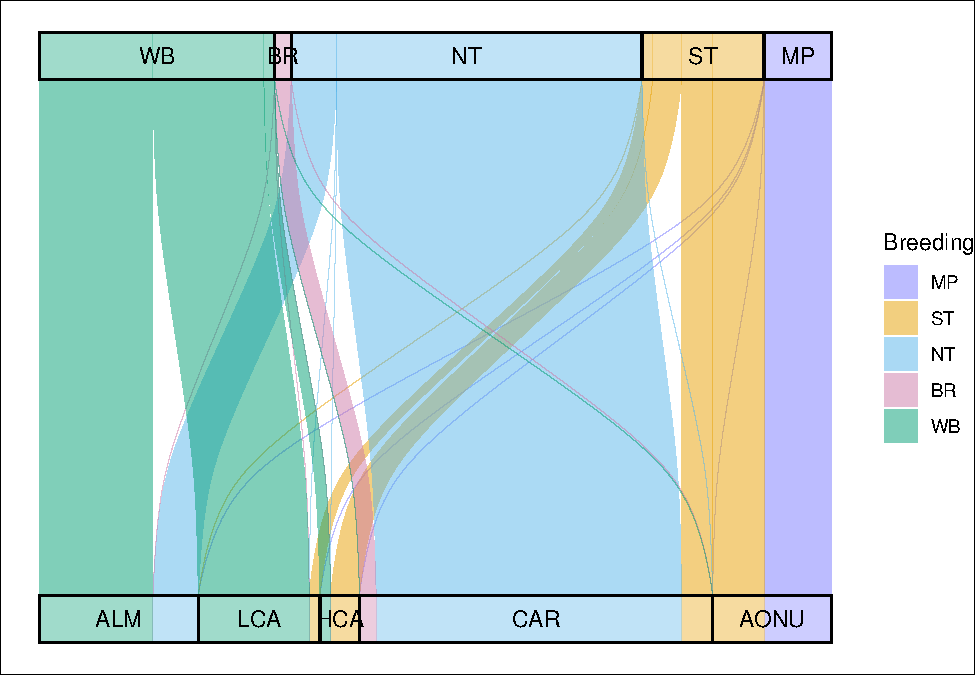
\includegraphics{Mignette_files/figure-latex/unnamed-chunk-24-1.pdf}

In this visualization, node size corresponds to the amount of connectivity with that population and edge size corresponds to the amount of connectivity between the populations. By default, breeding populations are in the top row (red) and nonbreeding populations are in the bottom row (blue).

We also can change the \texttt{connected\_tol} threshold in the \texttt{net\_create} function to not output extremely weak connectivity. For example, the plot below removes connectivity less than 0.02:

\begin{Shaded}
\begin{Highlighting}[]
\NormalTok{net }\OtherTok{\textless{}{-}}\NormalTok{ mignette}\SpecialCharTok{::}\FunctionTok{net\_create}\NormalTok{(mignette}\SpecialCharTok{::}\NormalTok{amre\_conn, }
                            \AttributeTok{node.names =} \FunctionTok{list}\NormalTok{(bnode\_names, wnode\_names),}
                            \AttributeTok{connected\_tol =} \FloatTok{0.02}\NormalTok{) }\CommentTok{\# threshold}
\NormalTok{net}\SpecialCharTok{$}\NormalTok{display\_par}\SpecialCharTok{$}\NormalTok{node\_size\_scale}\OtherTok{\textless{}{-}}\FunctionTok{c}\NormalTok{(}\DecValTok{5}\NormalTok{,}\DecValTok{20}\NormalTok{)}
\NormalTok{net}\SpecialCharTok{$}\NormalTok{display\_par}\SpecialCharTok{$}\NormalTok{edge\_size\_scale}\OtherTok{\textless{}{-}}\FunctionTok{c}\NormalTok{(}\DecValTok{1}\NormalTok{,}\DecValTok{5}\NormalTok{)}
\FunctionTok{plot}\NormalTok{(mignette}\SpecialCharTok{::}\FunctionTok{net\_draw}\NormalTok{(net))}
\end{Highlighting}
\end{Shaded}

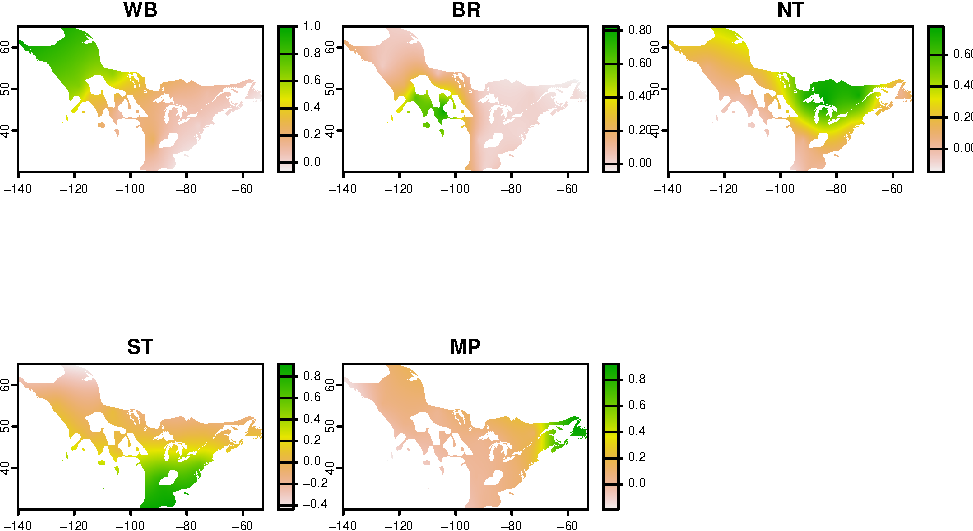
\includegraphics{Mignette_files/figure-latex/unnamed-chunk-25-1.pdf}

This sums up the basics of creating and visualizing a migratory network. We encourage users to explore and build upon the visualization tools we provide (e.g.~overlay the migratory networks on geographic ranges) - the options are endless, enjoy!

\hypertarget{other-visualization-options}{%
\section{Other visualization options}\label{other-visualization-options}}

Ok, we'll toss out another way to visualize these networks using the \href{https://cran.r-project.org/web/packages/ggalluvial/vignettes/ggalluvial.htm}{\texttt{ggalluvial} package} because it's really fun.

\begin{Shaded}
\begin{Highlighting}[]
\FunctionTok{library}\NormalTok{(tidyverse)}
\FunctionTok{library}\NormalTok{(mignette)}
\FunctionTok{library}\NormalTok{(ggalluvial)}

\NormalTok{bnode\_names }\OtherTok{\textless{}{-}} \FunctionTok{c}\NormalTok{(}\StringTok{"WB"}\NormalTok{, }\StringTok{"BR"}\NormalTok{, }\StringTok{"NT"}\NormalTok{, }\StringTok{"ST"}\NormalTok{, }\StringTok{"MP"}\NormalTok{)}
\NormalTok{wnode\_names }\OtherTok{\textless{}{-}} \FunctionTok{c}\NormalTok{(}\StringTok{"ALM"}\NormalTok{, }\StringTok{"LCA"}\NormalTok{, }\StringTok{"HCA"}\NormalTok{, }\StringTok{"CAR"}\NormalTok{, }\StringTok{"AONU"}\NormalTok{)}

\NormalTok{cluster\_colors }\OtherTok{\textless{}{-}}  \FunctionTok{c}\NormalTok{(}
  \StringTok{\textasciigrave{}}\AttributeTok{ST}\StringTok{\textasciigrave{}} \OtherTok{=} \StringTok{"\#FF99FF"}\NormalTok{, }\CommentTok{\# pink/Southern Temperate}
  \StringTok{\textasciigrave{}}\AttributeTok{BR}\StringTok{\textasciigrave{}} \OtherTok{=} \StringTok{"\#3399FF"}\NormalTok{, }\CommentTok{\# blue/Basin Rockies}
  \StringTok{\textasciigrave{}}\AttributeTok{NT}\StringTok{\textasciigrave{}} \OtherTok{=} \StringTok{"\#FFFF33"}\NormalTok{, }\CommentTok{\# yellow/Northern Temperate}
  \StringTok{\textasciigrave{}}\AttributeTok{WB}\StringTok{\textasciigrave{}} \OtherTok{=} \StringTok{"\#339933"}\NormalTok{, }\CommentTok{\# green/Western Boreal}
  \StringTok{\textasciigrave{}}\AttributeTok{MP}\StringTok{\textasciigrave{}} \OtherTok{=} \StringTok{"\#CC0033"} \CommentTok{\# red/Maritime Provinces}
\NormalTok{) }

\NormalTok{amre\_conn\_df }\OtherTok{\textless{}{-}}\NormalTok{ mignette}\SpecialCharTok{::}\NormalTok{amre\_conn }\SpecialCharTok{\%\textgreater{}\%}
  \FunctionTok{as\_tibble}\NormalTok{(}\AttributeTok{rownames =} \StringTok{"Breeding"}\NormalTok{) }\SpecialCharTok{\%\textgreater{}\%}
  \FunctionTok{pivot\_longer}\NormalTok{(}\AttributeTok{cols =}\NormalTok{ ALM}\SpecialCharTok{:}\NormalTok{AONU, }\AttributeTok{names\_to =} \StringTok{"Nonbreeding"}\NormalTok{, }\AttributeTok{values\_to =} \StringTok{"Connectivity"}\NormalTok{) }\SpecialCharTok{\%\textgreater{}\%}
  \FunctionTok{mutate}\NormalTok{(}\AttributeTok{Connectivity =} \FunctionTok{ifelse}\NormalTok{(Connectivity }\SpecialCharTok{\textless{}} \FloatTok{0.01}\NormalTok{, }\DecValTok{0}\NormalTok{, Connectivity)) }\SpecialCharTok{\%\textgreater{}\%}
  \FunctionTok{mutate}\NormalTok{(}\AttributeTok{Breeding =} \FunctionTok{factor}\NormalTok{(Breeding, }\AttributeTok{levels =} \FunctionTok{rev}\NormalTok{(bnode\_names)),}
         \AttributeTok{Nonbreeding =} \FunctionTok{factor}\NormalTok{(Nonbreeding, }\AttributeTok{levels =} \FunctionTok{rev}\NormalTok{(wnode\_names)))}

\NormalTok{p.alluvial }\OtherTok{\textless{}{-}} \FunctionTok{ggplot}\NormalTok{(amre\_conn\_df,}
       \FunctionTok{aes}\NormalTok{(}\AttributeTok{y =}\NormalTok{ Connectivity, }\AttributeTok{axis1 =}\NormalTok{ Nonbreeding, }\AttributeTok{axis2 =}\NormalTok{ Breeding)) }\SpecialCharTok{+}
  \FunctionTok{geom\_alluvium}\NormalTok{(}\FunctionTok{aes}\NormalTok{(}\AttributeTok{fill =}\NormalTok{ Breeding), }\AttributeTok{width =} \DecValTok{1}\SpecialCharTok{/}\DecValTok{12}\NormalTok{) }\SpecialCharTok{+}
  \FunctionTok{scale\_fill\_manual}\NormalTok{(}\AttributeTok{values =}\NormalTok{ cluster\_colors) }\SpecialCharTok{+}
  \FunctionTok{geom\_stratum}\NormalTok{(}\AttributeTok{alpha =} \FloatTok{0.25}\NormalTok{, }\AttributeTok{width =} \DecValTok{1}\SpecialCharTok{/}\DecValTok{12}\NormalTok{) }\SpecialCharTok{+}
  \FunctionTok{geom\_text}\NormalTok{(}\AttributeTok{stat =} \StringTok{"stratum"}\NormalTok{, }\FunctionTok{aes}\NormalTok{(}\AttributeTok{label =} \FunctionTok{after\_stat}\NormalTok{(stratum))) }\SpecialCharTok{+}
  \FunctionTok{scale\_x\_discrete}\NormalTok{(}\AttributeTok{limits =} \FunctionTok{c}\NormalTok{(}\StringTok{"Nonbreeding"}\NormalTok{, }\StringTok{"Breeding"}\NormalTok{),}
                   \AttributeTok{expand =} \FunctionTok{c}\NormalTok{(}\FloatTok{0.05}\NormalTok{, }\FloatTok{0.05}\NormalTok{)) }\SpecialCharTok{+} 
  \FunctionTok{coord\_flip}\NormalTok{() }\SpecialCharTok{+}
  \FunctionTok{theme\_void}\NormalTok{() }\SpecialCharTok{+}
  \FunctionTok{theme}\NormalTok{(}\AttributeTok{plot.background =} \FunctionTok{element\_rect}\NormalTok{(}\AttributeTok{fill =} \StringTok{"white"}\NormalTok{))}

\NormalTok{p.alluvial}
\end{Highlighting}
\end{Shaded}

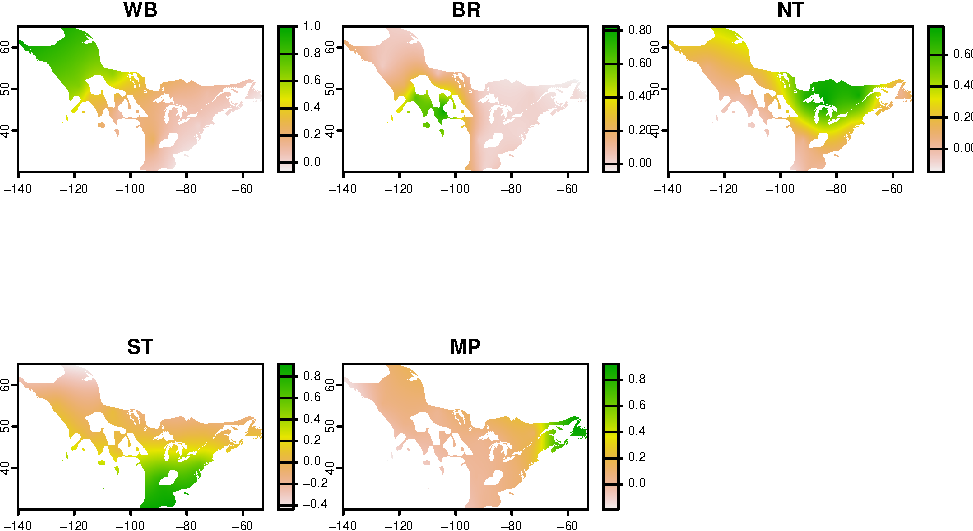
\includegraphics{Mignette_files/figure-latex/unnamed-chunk-26-1.pdf}

  \bibliography{book.bib,packages.bib}

\end{document}
